%!TEX root = ../thesis.tex
% ******************************* Thesis Appendix B ********************************

\chapter{Hardware Triggering At SBND} 
\label{appendix_hardware_trigger}
\ifpdf
    \graphicspath{{Appendix1/Figs/Raster/}{Appendix1/Figs/PDF/}{Appendix1/Figs/}}
\else
    \graphicspath{{Appendix1/Figs/Vector/}{Appendix1/Figs/}}
\fi

The hardware triggering at SBND was previously discussed in Chapter \ref{ChapterDetector} Sec. \ref{sec:sbnd_trigger}.
Here a detailed description of the trigger signal distribution is provided.
Fig. \ref{fig:SBND_Trigger} depicts the flow chart of signal inputs and outputs to and from the PTB, shown as the pink box, across different subsystems.  
The PTB receives the beam signal from the beam subsystem, shown as the green box.
The beam signal denoted as \textit{early warning} informs the PTB about the status of the BNB beam, indicating whether the beam has arrived at the detector hall.
Also shown by the green box is the White Rabbit timing subsystem that distributes the Pulse Per Second (PPS) and 10 MHz clock signals to the PTB and other subsystems to maintain synchronisation.
The White Rabbit timing, as part of the triggering and DAQ, was be discussed in detail in Chapter \ref{ChapterDAQ}.

From the detection subsystems, the input signals to the PTB are from PMTs and CRTs.
The PMTs provide information regarding the energy deposited inside the detector and whether its magnitude and location are consistent with a neutrino-induced event.
The readouts of the PMTs are CAENV1730SB digitizers, shown as the light blue boxes.
Each digitizer sends a \textit{majority trigger} directly to the PTB if its channels cross a threshold.
In addition, the number of channels above a threshold from the digitizers, denoted as \textit{board sums}, are directed to the Master Trigger Card Analog (MTC/A), shown as the red box.    
The MTC/A performs a simple logic gate calculation to determine the number of PMT pairs above a threshold, denoted as \textit{threshold crossing}, informing the PMT signal intensity and location.
This signal from the MTC/A is input directly to the PTB.  
On the other hand, signals from the CRTs for triggering are much simpler.
Coincident hits from any CRT walls, shown by the purple box, form \textit{CRT triggers}, which are input straight to the PTB.

Once a trigger is formed, the PTB send the trigger signals to subsequent readout subsystems to acquire the event, shown as the pink arrows leaving the PTB in Fig. \ref{fig:SBND_Trigger}.
An event contains two types of trigger signals: a single Event Trigger (ETRIG) and multiple Flash Triggers (FTRIGs).
The ETRIG is issued to the TPC readout, shown as the orange box labelled Nevis Trigger Board (Nevis TB) to acquire waveforms from the wire planes.
The FTRIGs are issued to the readouts of the PDS, shown as the light and dark blue boxes, to capture waveforms from the optical detectors.

An additional usage of the PTB is that it can output clock signals for some of the readout electronics.
For the Nevis TB of the TPC readouts, it sends a PPS signal that is locked to the PPS signal that it receives from the White Rabbit timing system.
This is depicted as the light pink arrow leaving the PTB to the Nevis TB.
Moreover, the PTB sends a T1 Reset to CRT readouts shown as the pink arrows leaving the PTB to CRT, of which the CRT T1 clock was detailed in Sec. \ref{sec4InternalClock}.
The T1 Reset signal here is locked to the early warning signal from the beam system with some added delay so that it occurs some time \textit{before} when the beam spill begins.
Originally, the T1 Reset signal to the CRT readouts was the BES signal from the beam system, which occurred \textit{right} when a beam spill begins.
Resetting the T1 clock enforces some dead time on CRT readouts.
Therefore, the T1 Reset signal was switched from the beam system to the PTB to have dead time outside of the beam spill window.  

\begin{figure}[hb!] 
\centering    
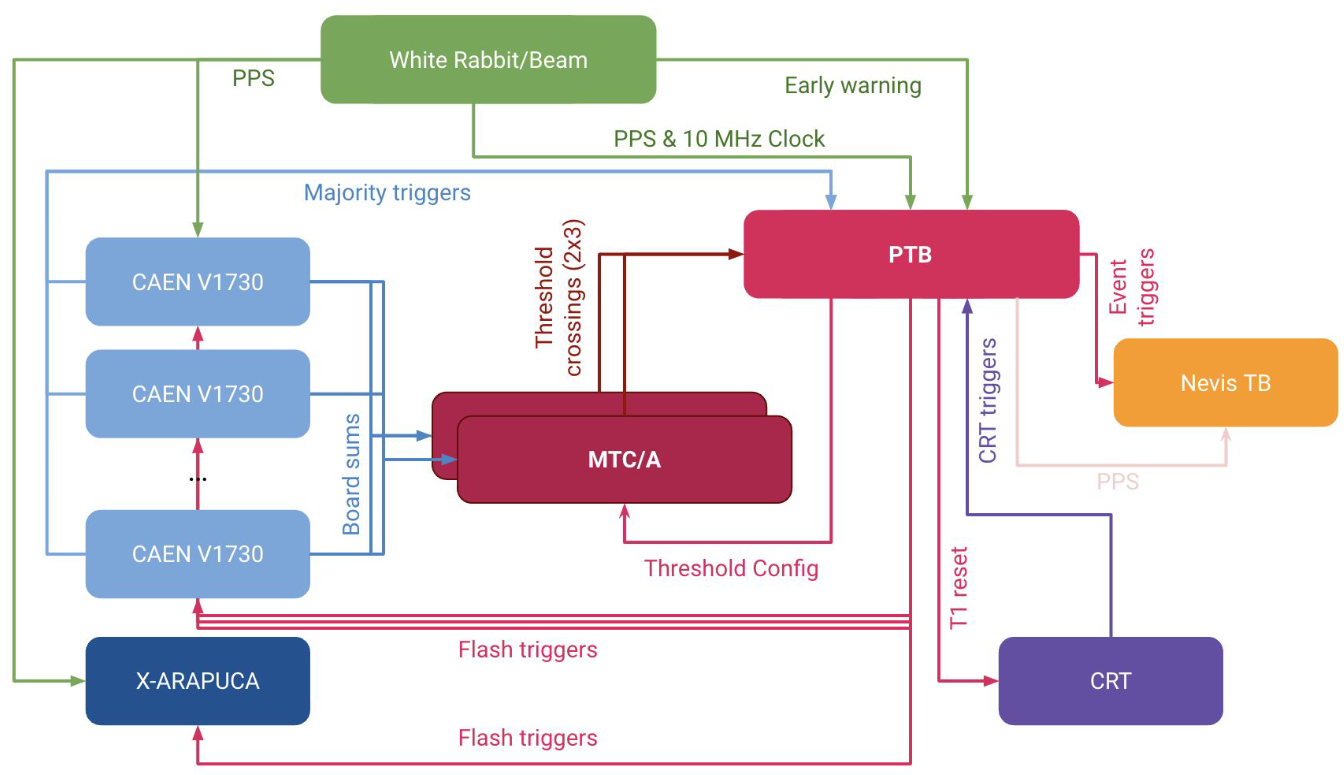
\includegraphics[width=1.0\textwidth]{SBND_Trigger}
\caption[Hardware Triggering Flow Chart]{
Flow chart showing the signal flow of the hardware triggering \cite{ptb_gvs}.
}
\label{fig:SBND_Trigger}
\end{figure}
